\section{Technisches}

\subsection{Formel vorstellen \& Variablen klären}
\subsubsection{Auffrischung:Sinus- und Kosinusfunktion mit Parametern}
Die einfachste Form eines Tons lässt sich durch eine Sinus- oder Kosinusschwingung beschreiben. Dabei handelt es sich mathematisch gesehen um eine Sinus- oder eine Kosinusfunktion. Beide gehören zu den trigonometrischen Funktionen, auch Winkelfunktionen genannt. Damit einige später folgende mathematische und für die FM-Synthese erforderliche Berechnungen besser verstanden werden können, wird hier kurz auf die Grundlagen zu Sinus- und Kosinus Funktionen eingegangen. 

Sinus und Kosinus sind periodische Funktionen, d.h. die Funktionswerte wiederholen sich nach einer sogenannten Periode. Mathematisch ausgedrückt muss es dafür eine konstante p  geben, für die bei einem beliebigen x gilt: $f(x + p) =  f(x)$ .

Am besten verdeutlichen kann man dies anhand des Einheitskreises. Abbildung \ref{fig:unitcircle} zeigt, wie sich Sinus und Kosinus aus den Seiten eines rechtwinkligen Dreiecks im Einheitskreis berechnen lassen:

\begin{figure} [ht]
\centering
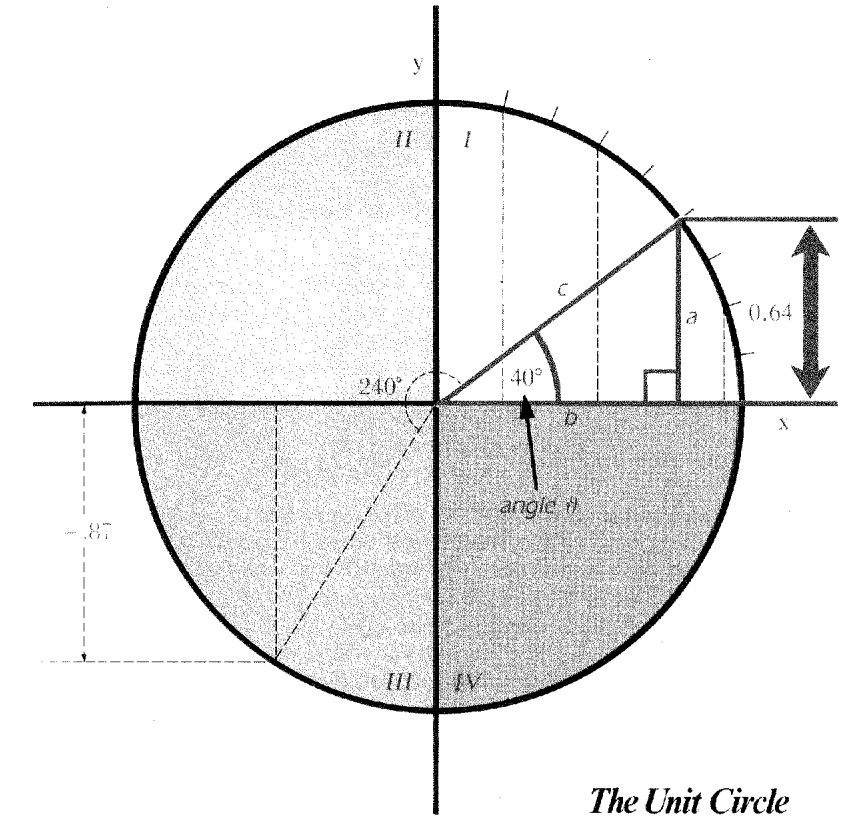
\includegraphics[width=0.95\textwidth]{Unit_Circle.png}
\caption{Der Einheitskreis}
\label{fig:unitcircle}
Quelle: FM: Theory and Application: Fig. 2.6
\end{figure}

Dabei gilt: 

$\sin(\pi) = \frac{\text{gegenüberliegende Seite}}{\text{Hypotenuse}} = \frac{a}{c}$, wobei die Hypotenuse im Einheitskreis eine Länge von 1 hat. 

$\to\sin(\pi) = \frac{a}{1} = a$.

$\cos(\pi) = \frac{\text{anliegende Seite}}{\text{Hypotenuse}} = \frac{b}{c} = \frac{b}{1} = b$.\\

\begin{figure} [ht]
\centering
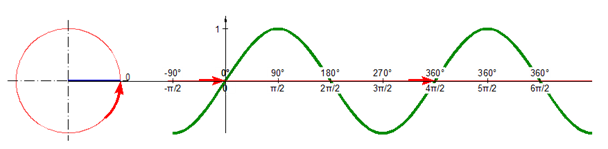
\includegraphics[width=0.95\textwidth]{sinus_einheitskreis.png}
\caption{Vom Einheitskreis zum Sinus}
\label{fig:unitcircleToSinus}
Quelle: \url{http://www.ulrich-rapp.de/stoff/mathematik/Sinus_Einheitskreis.gif}
\end{figure}

Die Sinusfunktion erhält man, wenn man auf der y-Achse lediglich die Funktionswerte des Kreises betrachtet und den Winkel im Einheitskreis als x-Werte der Funktion nimmt. Bei einer Schwingung wird für x dann die Zeit t eingesetzt. Eine Periode ist genau $2\pi$ Einheiten auf der Horizontalen Achse lang ($\pi$ ist die Kreiszahl), was im Einheitskreis einem Winkel von 360\degree entspricht. Daher spricht man auch von Winkelfunktionen, denn man kann den Funktionswert der Sinus- und Kosinusfunktion auch anhand des Winkels im Einheitskreis angeben. 
Eine Veranschaulichung des Zusammenhangs zwischen den Einheitskreis und der Sinusfunktion zeigt Abbildung \ref{fig:unitcircleToSinus}.

Der Unterschied von der Kosinusfunktion zur Sinusfunktion ist, dass der Kosinus bei dem Funktionswert 1 beginnt und Sinus bei Funktionswert 0. Aus diesem Zusammenhang lassen sich folgende Beziehungen zwischen Sinus und Kosinus feststellen:\\

\begin{lstlisting}[mathescape]
$\sin(\frac {\pi}{2} – x) =\cos(x)$
$\cos(\frac {\pi}{2} – x) = \sin(x)$
\end{lstlisting}

Überträgt man diese mathematischen Erkenntnisse nun auf einen Ton, so kann man dessen Funktion wie folgt beschreiben: 		$y(t) = y_0 * \sin(2 \pi f * t)$

Um 90\degree oder pi/2 verschoben gilt: 		$y(t) = y_0*\cos(2 \pi f*t)$

Bei $y_0$ handelt es sich um die Amplitude des Tons, also dessen Lautstärke. Alle Funktionswerte der Funktion werden mit diesem Faktor multipliziert und dadurch größer oder kleiner.

F ist die Frequenz des Tons. Sie gibt die Anzahl der Schwingungen (Perioden) pro Sekunde an und wird in $f=\frac{1}{T}$ angegeben, wobei T die Periodendauer ist. Die Einheit ist Herzt(Hz).
Je größer die Frequenz eines Tones ist, desto höher klingt er für das Ohr.

Für das menschliche Ohr hören sich beide Schwingungen gleich an, da diese lediglich um $\frac{1}{4}$ der Periode verschoben sind. 

\subsubsection{Erklärung: Trägerfrequenz, Modulationsfrequenz, Modulationsindex}

In diesem Kapitel wird auf die unterschiedlichen Parameter eingegangen, welche in der Formel der einfachen Frequenzmodulation vorkommen. Zudem wird deren Funktion im Einzelnen beschrieben.

Die Parameter werden mit der Gleichung in Sinus-Darstellung vorgestellt, d.h. Trägersignal und Modulator sind Sinus Funktionen. Dieselbe Erklärung funktioniert jedoch analog dazu auch mit Cosinus Funktionen für den Träger und den Modulator.
Die Gleichung für eine frequenzmodulierte Welle lautet wie folgt:
\[ e(t) = A sin(\alpha t + I sin(\beta t)) \]

\begin{lstlisting}[mathescape]
- $ e(t) $ beschreibt im die Amplitude des Modulierten Signals zum Zeitpunkt t.
- A stellt die höchste Amplitude des modulierten Signals dar. 
- $ \alpha $ ist die Frequenz des Träger Signals in Hertz (Schwingungen pro Sekunde)
- $ \beta $ ist die Frequenz des Modulators in Hertz (Schwingungen pro Sekunde). 
- I stellt den Modulationsindex dar. Dieser setzt sich wie folgt zusammen: $ I = \frac{d}{m} $ mit:
	= d: Frequenzhub der Modulation, d.h. der größte momentane Unterschied zwischen der Frequenz des Trägers und der des modulierten Signals.
	Auch: Frequenzänderung, welche durch die Modulation der Trägerfrequenz verursacht wird.
	= m: Frequenz des Modulators
\end{lstlisting}

Der Modulationsindex beschreibt also das Verhältnis des Frequenzhubs zur Modulationsfrequenz.
Man kann anhand der Formel bereits erkennen, dass bei einem Modulationsindex von 0 keine Modulation stattfindet. Dabei wird der Frequenzhub der Modulation auch gleich 0, da $ I=\frac{d}{m} $ und somit $ d = 0*m = 0 $ gilt. 
\[ e(t) = A \sin(\alpha t + 0 \sin(\beta t))  \Rightarrow  e(t) = a \sin(\alpha t) \]
Anhand der Frequenz des Modulators kann man sehen, wie oft der oben beschriebene Frequenzhub pro Sekunde durchlaufen wird. Beispiel: Bei einer Modulatorfrequenz von 440 Hz wird der Frequenzhub 440 mal pro Sekunde durchlaufen.
